\chapter{Programmbeschreibung}
\label{chap:Programmbeschreibung}
\todo[inline]{hier noch ein paar einleitende Sätze}


\section{Parameter des Fluggeräts}
\label{sec:parameter_fluggeraet}
Bei der Auslegung des Fluggeräts werden nicht nur Multicopter betrachtet sondern auch Flächenflugzeuge, sogenannte fixed wing UAVs. Aus diesem Grund werden die Parameter Motor, Propeller, Batterie und Umgebungsparameter allgemein für beide Arten der UAVs festgelegt. Anschließend werden die Parameter des Multicopters oder des Flächenflugzeugs zur Charakterisierung dieser bestimmt, je nachdem, welches Fluggerät untersucht werden soll. Im Anschluss werden die Formeln der Leistungsberechnung dargelegt. 
Das Programm und die diesem grundlegende Leistungsberechnung, basieren auf dem internen Bericht \todo[inline]{ fix das Problem mit "Leistungsberechnung von Multicoptern" von Y. Beyer (2016) Blub}. Aus dieser wurden die Berechnung der Aerodynamik von Multicoptern, die Pulsweitenmodulation und der Batterieentladung sowie die festgelegten Grenzen der fliegbaren Flugzustände übernommen. \\

 
\subsubsection{Flugsystem}
Zu Beginn der Mission muss das Flugsystem festgelegt werden, da die Berechnung der Aerodynamik entscheidend vom Flugsystem abhängt ist. Die Abfrage erfolgt mit der Variablen \texttt{Abfrage\_Flugsystem}. Diese kann die Werte \texttt{1} für einen Multicopter oder \texttt{0} für ein Flächenflugzeug annehmen.

\subsubsection{Motor}
Die ersten drei Motorparameter in Tab. \ref{tab:mot_parameter} sind notwendig, um den Motorzustand zu berechnen. Der vorletzte Parameter dient als technische Grenze, die für ein gut ausgelegtes System nicht überschritten wird. Die Motormasse fließt in Kombination mit der Anzahl der Propeller in die Gesamtmasse des Fluggerätes mit ein. Die vorrangige technische Leistungsgrenze ist ist die maximale Motorleistung, die durch den maximalen Motorstrom \ensuremath{I_{max}} repräsentiert wird.
\todo[inline]{Quelle für AXI Datenbank}

\begin{center}
	\captionof{table}{Motorparameter für technische Grenzen}
	\begin{tabular}{l l l} \hline
		 Parameter & Variablenname & Einheit \\ \hline
		 Innenwiderstand \ensuremath{R_i} & \texttt{R\_i} & \SI{}{\ohm} \\
		 Geschwindigkeitskonstante \ensuremath{K_V} & \texttt{K\_V} & \ensuremath{\frac{RPM}{V}} bzw. \ensuremath{\frac{U}{Vs}} \\
		 Leerlaufstrom \ensuremath{I_0} & \texttt{I\_O} & \ensuremath{A}  \\
		 maximaler Dauerstrom \ensuremath{I_{max}} & \texttt{I\_max} & \ensuremath{A} \\
		 Motormasse \ensuremath{m_{Mot}} & \texttt{m\_Mot} & \ensuremath{kg} \\ \hline
	\end{tabular}	
	\label{tab:mot_parameter}
\end{center}

\subsubsection{Propeller}
Der Propellername wird in der Form 'Durchmesser x Steigung' angegeben (siehe Tab. \ref{tab:prop_parameter}). Der Name ist wichtig, um das Propellerkennfeld aus der Propellerdatenbank von APC \todo[inline]{Quelle für APC angeben} zu entnehmen. Die Anzahl der Propeller beeinflusst entscheidend die Geometrie des Fluggerätes. Weiterhin wird damit der benötigte Schub auf die Anzahl der Propeller aufgeteilt. Die letzten Parameter dienen zur Bestimmung der Effekte einer Anströmung und damit der Berücksichtigung der Blattelemententheorie.

\begin{center}
	\captionof{table}{Propellerparameter für Schub, aerodynamische und technische Grenzen}
	\begin{tabular}{l l l} \hline
		 Parameter & Variablenname & Einheit \\ \hline
		 Propellername & \texttt{prop\_name} & \ensuremath{-} \\
		 Anzahl der Propeller \ensuremath{n_{Prop}} & \texttt{n\_Prop} & \ensuremath{-} \\ \hline
	\end{tabular}	
	\label{tab:prop_parameter}
\end{center}

\subsubsection{Batterie}
Die in Tab. \ref{tab:bat_parameter} aufgeführten Parameter der Batterie bestimmen zum einen die verfügbare Kapazität und zum anderen die Batterieentladung. Bei der Energiedichte handelt es sich um repräsentative Werte für den verwendeten Akkutyp, z.B. Li-Ion oder Li-Po. \todo[inline]{Quelle für die Energiedichte von LI-Ion Batterien heraussuchen}. Die minimale Zellenspannung ist ein Erfahrungswert, der am \textit{Institut für Flugführung} verwendet wird. Um den Energieverlust der Batterie zu berechnen, wird die Peukert-Konstante herangezogen. Diese beträgt für Li-Po-Akkus ca. $1,01 \leq P \leq 1,05$ und für Li-Ion-Akkus ca. 1,05 (\textcolor{red}{Traub} Blub). Außerdem ist die Peukert-Konstante für Li-Po-Batterien von der Temperatur abhängig. Niedrigere Temperaturen als die Umgebungstemperatur können die angegebene Nennkapazität reduzieren und die Batterieverluste progressiv steigen lassen. Die maximale C-Rate dient als weitere technische Begrenzung, die wiederum für ein gut ausgelegtes System nicht erreicht wird.

\begin{center}
	\captionof{table}{Batterieparameter zur Berechnung der verbleibenden Restladung sowie der technischen Grenzen}
	\begin{tabular}{l l l} \hline
		 Parameter & Variablenname & Einheit \\ \hline
		 Energiedichte \ensuremath{\frac{E_{Bat}}{m_{Bat}}}& \texttt{E\_Dichte} & \SI{940000}{J/kg} \\
		 Anzahl der Batteriezellen \ensuremath{N_{Bat,cell}} & \texttt{N\_bat\_cell} & \ensuremath{-} \\
		 nominale Spannung pro Batteriezelle \ensuremath{U_{Bat,cell}} & \texttt{U\_bat\_nom} & \SI{3,7}{V} \\
		 minimale Spannung pro Batteriezelle \ensuremath{U_{Bat,cell,min}} & \texttt{U\_bat\_min} & \SI{3,1}{V} \\
		 Peukert-Konstante \ensuremath{P}& \texttt{P\_bat\_Peukert} & \ensuremath{1,05} \\
		 Maximale C-Rate \ensuremath{C_{Rate,max}} & \texttt{C\_Rate\_max} & \ensuremath{-} \\
		 Batteriemasse \ensuremath{m_{Bat}} & \texttt{m\_bat} & \SI{}{kg} \\ \hline
	\end{tabular}	
	\label{tab:bat_parameter}
\end{center}
\todo[inline]{Fehlen hier Parameter der Normzelle}

\subsubsection{Multicopter}
Die Parameter für den Multicopter sind in Tab. \ref{tab:multicop_parameter} aufgeführt. Die Leermasse fließt mit in die Gesamtmasse mit ein und wird für die Berechnung des Schubs und weiterer Parameter benötigt. Die Beiwerte sind reine Schätzwerte. Für die nachfolgenden Berechnungen ist nur die obere Stirnfläche von Bedeutung, da sich auf diese die Beiwerte als Referenzfläche beziehen. Die Propeller bleiben bei den Stirnflächen unberücksichtigt.
\begin{center}
	\captionof{table}{Parameter des Multicopters}
	\begin{tabular}{l l l} \hline
		 Parameter & Variablenname & Einheit \\ \hline
		 Leermasse des Multicopters \ensuremath{m_{Copter}} & \texttt{m\_copter} & \ensuremath{kg}\\
		 Obere Stirnfläche \ensuremath{A_{copter,oben}} & \texttt{A\_copter} & \ensuremath{m^2}\\
		 seitliche Stirnfläche \ensuremath{A_{copter,seitlich}} & \texttt{A\_copter\_seitlich} & \ensuremath{m^2}\\
		 Oberer Widerstandsbeiwert \ensuremath{c_{W,copter,oben}} & \texttt{c\_W\_copter\_oben} & \ensuremath{-}\\
		 Seitlicher Widerstandsbeiwert \ensuremath{c_{W,copter,seitlich}} & \texttt{c\_W\_copter\_seitlich} & \ensuremath{-}\\
		 Maximaler Auftriebsbeiwert \ensuremath{c_{A,copter,max}} & \texttt{c\_A\_copter\_max} & \ensuremath{-}\\ \hline
	\end{tabular}	
	\label{tab:multicop_parameter}
\end{center}

\subsubsection{Flächenflugzeug}
Mit der Leermasse wird analog zum Multicopter der Schub berechnet. Der zweite Parameter wird zur Bestimmung des aktuellen Flugzustandes benötigt. Dieser ergibt sich aus einem Auslegungszustand mit vorgegebener Gleitzahl \ensuremath{E^\star} und Geschwindigkeit \ensuremath{V^\star} in Bodennähe. Die Bodennähe und die Höhe sind entsprechend durch die Dichte charakterisiert.
\begin{center}
	\captionof{table}{Parameter des Flächenflugzeug}
	\begin{tabular}{l l l} \hline
		 Parameter & Variablenname & Einheit \\ \hline	 
		 Leermasse des Flächenflugzeug \ensuremath{m_{Flugzeug}}& \texttt{m\_Flugzeug} & \ensuremath{kg}\\ 
		 Gleitzahl \ensuremath{E} & \texttt{E} & \ensuremath{-}\\	
		 Auslegungsgleitzahl \ensuremath{E^\star} & \texttt{E\_stern} & \ensuremath{-}\\
		 Auslegungsgeschwindigkeit \ensuremath{V^\star} & \texttt{V\_stern} & \ensuremath{m/s}\\
		 Auslegungshöhe \ensuremath{\rho^\star} & \texttt{rho\_stern} & \SI{1,225}{kg/m^3}\\ \hline
	\end{tabular}	
	\label{tab:flugzeug_parameter}
\end{center}
Zusätzlich wird noch der Bahnneigungswinkel \ensuremath{\gamma} für jeden Höhenschritt diskretisiert. Dabei sollte die Schrittweite so klein wie nötig gewählt werden, um die Genauigkeit zu maximieren und so groß wie möglich, um die Rechendauer akzeptabel kurz zu halten. Der Maximalwert entspricht in diesem Fall einem senkrechten Steigflug.
\begin{center}
	\captionof{table}{Diskretisierung des Bahnneigungswinkels}
	\begin{tabular}{l l l} \hline
		 Parameter & Variablenname & Einheit \\ \hline	  
		 Kleinster Bahnneigungswinkel \ensuremath{\gamma_{min}} & \texttt{gamma\_min} & \SI{1}{^\circ}\\	
		 Schrittweite des Bahnneigungsw. \ensuremath{\Delta\gamma} & \texttt{gamma\_Delta} & \SI{1}{^\circ}\\
		 Größter Bahnneigungswinkel \ensuremath{\gamma_{max}} & \texttt{gamma\_max} & \SI{90}{^\circ}\\ \hline
	\end{tabular}	
	\label{tab:flugzeug_parameter}
\end{center}


\section{Parameter der Mission}
\label{sec:parameter_mission}

\subsubsection{Missionsparameter}
Innerhalb der Flugparameter kann die Nutzlast \texttt{m\_Nutz} des Fluggerätes bestimmt werden. Diese Masse fließt mit der Masse des Fluggerätes, der der Motoren sowie der der Batterie in die Gesamtmasse mit ein. Im Rahmen des Projektes AEROMET UAV ist die Nutzlast auf \SI{250}{g} festgelegt.
 
\subsubsection{Flugbahnparameter}
Die Flugbahnparameter geben für den Multicopter den Bahnneigungswinkel sowie die Bahngeschwindigkeit vor. Der Bahnneigungswinkel ist mit einem Wert von \ensuremath{90^\circ} festgelegt, was einem vertikalen Steigflug nach oben entspricht.
\begin{center}
	\captionof{table}{Flugbahnparameter}
	\begin{tabular}{l l l} \hline
		 Parameter & Variablenname & Einheit \\ \hline
		 Bahngeschwindigkeit \ensuremath{V_{Kg}} & \texttt{V\_Kg} & \ensuremath{m/s}\\		 
		 Bahnneigungswinkel \ensuremath{\gamma_{Copter}}& \texttt{gamma\_copter} & \ensuremath{^\circ}\\ \hline
	\end{tabular}	
	\label{tab:flugparameter}
\end{center}

\subsubsection{Umgebungsparameter und Diskretisierung variabler Umgebungsparameter}
Die Erdbeschleunigung und der Adiabatenexponent werden als konstant über der Höhe angenommen. Mit Startwerten für die Höhe, die Temperatur, die Dichte und des Luftdrucks werden die Abflugbedingungen am Abflugort spezifiziert.  Die Schrittweite der Höhe legt die Genauigkeit der Höhendiskretisierung fest.
\begin{center}
	\captionof{table}{Umgebungsparameter}
	\begin{tabular}{l l l} \hline
		 Parameter & Variablenname & Einheit \\ \hline
		 Erdbeschleunigung \ensuremath{g} & \texttt{g} & 9,81 \ensuremath{m/s^2} \\
		 Starthöhe \ensuremath{H_0} & \texttt{H\_0} & \ensuremath{m} \\
		 Schrittweite der Höhe  \ensuremath{\Delta H} & \texttt{Delta\_H} & \ensuremath{m} \\
		 maximale Höhe \ensuremath{H_{max}} & \texttt{H\_max} & \ensuremath{m} \\
		 Umgebungstemperatur am Start \ensuremath{T_0} & \texttt{T\_0} & \ensuremath{K} \\
		 Luftdruck am Start \ensuremath{p_0} & \texttt{p\_0} & \ensuremath{N/m^2} \\
		 Dichte am Start \ensuremath{\rho_0} & \texttt{rho\_0} & \ensuremath{kg/m^3} \\
		 Adiabatenexponent \ensuremath{\kappa} & \texttt{kappa} & \SI{1,4}{} \\
		 Windgeschwindigkeit \ensuremath{u_{Wg}} & \texttt{u\_Wg} & \ensuremath{m/s} \\ \hline
	\end{tabular}	
	\label{tab:umgebungs_parameter}
\end{center}

\section{Berechnung weiterer Parameter}
\begin{center}
	\captionof{table}{Berechnung weiterer Parameter}
	\begin{tabular}{l l l} \hline
		 Parameter & Variablenname & Gleichung\\ \hline
		 Nominale Batteriespannung & \texttt{U\_Bat\_nom} & \ensuremath{U_{Bat,nom} = N_{Bat,cell}\cdot U_{Bat,cell}} \\
		 Minimale Batteriespannung & \texttt{U\_Bat\_min} & \ensuremath{U_{Bat,min} = N_{Bat,cell}\cdot U_{Bat,cell,min}} \\
		 Propellerradius & \texttt{R} & \ensuremath{R = D\cdot 0,0254/2} \\
		 Fläche eines Propellers & F & \ensuremath{F = \pi\cdot R^2} \\
		 Temperatur in \SI{11}{km} Höhe & \texttt{T\_11} & \ensuremath{T_{11} = T_0 - 0.0065\cdot(11000-H_0)} \\
		 Dichte in \SI{11}{km} Höhe & \texttt{rho\_11} & \ensuremath{\rho_{11} = \rho_0\cdot\Big(1 - 0.0065\cdot\frac{11000}{T_0}\Big)^{4.256}} \\
		 Druck in \SI{11}{km} Höhe & \texttt{p\_11} & \ensuremath{p_{11} = p_0\cdot\Big(1 - 0.0065\cdot\frac{11000}{T_0}\Big)^{5.256}} \\ \hline
	\end{tabular}	
	\label{tab:umgebungs_parameter}
\end{center}


\newpage
\section{Aufbau des Programms}
\label{sec:aufbau_des_programms}
Der Aufbau des \textsc{Matlab}-Skriptes wird in den unteren Struktogrammen verdeutlicht. 
Abb. \ref{abb:programmstruktur} legt die Ablaufstruktur dar.
\todo[inline]{genauere Programmbeschreibung}
\begin{center}
\begin{figure}[H]
\begin{struktogramm}(163,153)
\assign[1]{Fluggerät auswählen und Komponenten definieren(im Startskript)}
\assign[1]{Missions- und Umgebungsparameter festlegen (im Startskript)}
\assign[1]{Diskretisierungen festlegen}
\assign[1]{Aufruf des Hauptskripts: Leistungsberechnung starten}
\assign[1]{Initialisierung der Parameterberechnung}
\while[5]{F\"ur alle Höhenabschnitte}
	\assign[1]{H\"ohe, Dichte, Luftdruck Temperatur berechnen}
	\assign[1]{arithmetische Mittelwert berechnen}
	\assign[1]{Schub- und Leistungskennfeld anpassen}
	\assign[2]{Initialisierung der Leistungsberechnung}
	\while[5]{Für alle Bahnneigungswinkel}
		\assign[2]{\textbf{Leistungsberechnung}}
	\whileend
	\ifthenelse[10]{1}{5}{Fluggerät?}{Multicopter (1)}{Flächenflugzeug (0)}
		\assign[2]{Übergabe der zwischengespeicherten Leistungsparameter}
		\change
		\ifthenelse[10]{5}{1}{Sind die Werte NaN?}{nein}{ja}
			\while[5]{Solange Abbruchkriterium nicht erreicht}		
				\assign[2]{Finde den Index mit der geringsten verbrauchten Energiemenge}
				\ifthenelse[10]{1}{1}{Werte innerhalb Leistungsgrenzen?}{ja}{nein}
				\assign[2]{Verlasse Schleife}
				\change
				\assign[2]{Suche nächst kleinere Energiemenge}
				\ifend
			\whileend
			\assign[2]{Übergabe aller Leistungsparameter mit diesem Index}
			\change
			\assign[2]{Verwerfe alle Ergebnisse}
		\ifend
	\ifend
\whileend
\assign[2]{Ergebnisse der Leistungsparameter in Diagrammen speichern}
\assign[2]{Speichern der Diagramme in .pdf-Datei}
\end{struktogramm}
\caption{Programmstruktur des MATLAB-Skripts}
\label{abb:programmstruktur}
\end{figure}
\end{center}

und Abb. \ref{abb:leistungsberechnung} veranschaulicht dem Programm zugrunde gelegten Ablauf der Leistungsberechnung.

\begin{center}
\begin{figure}[H]
\begin{struktogramm}(163,140)
\ifthenelse[15]{1}{1}{Flugger\"at?}{Multicopter (1)}{Fl\"achenflugzeug (0)}
			\assign[2]{Berechne Gesamtmasse}
			\assign[2]{Flugzeit für Höhenschritt berechnen}			
			\while[5]{Solange Abbruchkriterium nicht erreicht}
				\assign{Aerodynamik berechnen}
			\whileend
			\assign[2]{Schub berechnen}
			\change
			\assign[2]{Berechne Gesamtmasse}
			\assign[2]{Schub aus Bahnneigungswinkel und Auslegungspunkt berechnen}
			\assign[2]{Flugzeit für Höhenschritt berechnen}
		\ifend
		\assign[2]{Schub auf Propeller verteilen}
		\ifthenelse[10]{1}{4}{Schub zu gro\ss{}?}{ja}{nein}
			\assign[2]{Ergebnis verwerfen (NaN)}
			\change
			\assign[2]{Drehzahl und Drehmoment aus Propellerkennfeld interpolieren}
			\assign[2]{Motorzustand berechnen}
			\assign[2]{Zustand der Motorregler berechnen}
			\assign[2]{Zustand der Batterie neu berechnen}
			\assign[2]{Gesamtwirkungsgrad berechnen}
		\ifend
		\ifthenelse[10]{1}{1}{Werden Grenzen überschritten?}{ja}{nein}
			\assign[2]{Ergebnis verwerfen (NaN)}
			\change
			\assign[2]{Ergebnis beibehalten}
		\ifend
		\ifthenelse[10]{1}{1}{Fluggerät?}{Multicopter (1)}{Flächenflugzeug (0)}
			\assign[2]{break}
			\change
			\assign[2]{Speichern der aufgebrachten Energiemenge}
		\ifend
\end{struktogramm}
\caption{Programmstruktur des MATLAB-Skripts}
\label{abb:leistungsberechnung}
\end{figure}
\end{center}


%\begin{figure}[H]
%\centering
%	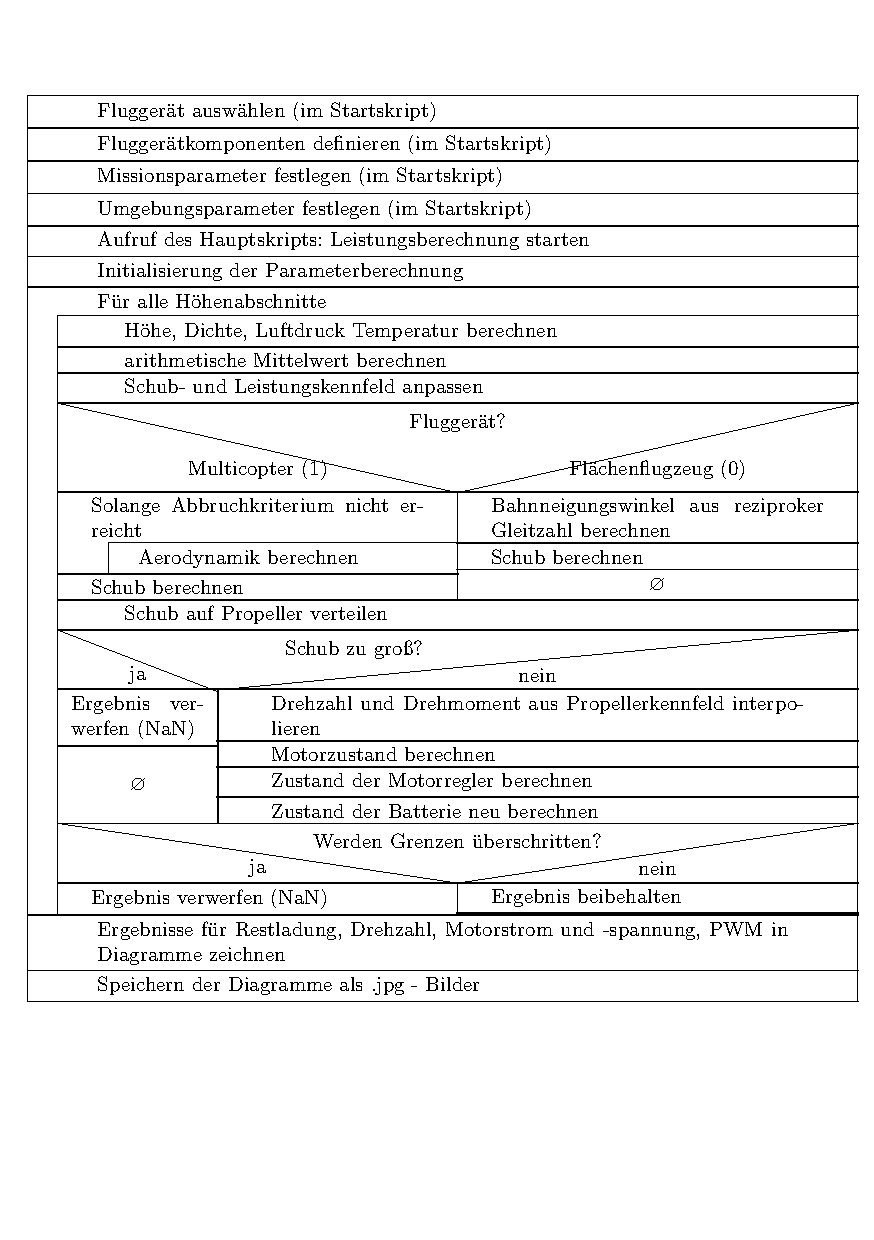
\includegraphics{Struktogramm/Struktogramm.pdf}
%	\caption{Struktogramm des MATLAB-Skripts}
%	\label{abb:struktogramm}
%\end{figure}


\section{Flugleistungsberechnung}
\label{sec:flugleistungsberechnung}
Die Leistungsberechnung ist umgekehrt zu einem realen Fluggerät aufgebaut. Die Berechnung startet bei der Ermittlung des benötigten Schubes für eine vorgegebene Fluggeschwindigkeit innerhalb eines aerodynamischen Modells. Mit diesem werden aus einem Propellerkennfeld die Drehzahl und das Drehmoment des Propellers bestimmt, welche den Motorzustand definieren. Die Motorzustandsgrößen legen wiederum zum einen die Pulsweitenmodulation und den Wirkungsgrad des Reglers fest und zum anderen fließen sie mit diesen Werten in die Berechnung der Batterierestladung ein. Zusammengenommen handelt es sich hierbei um ein statisches Modell. Dies steht dem realen, dynamischen Fluggerät gegenüber. Bei diesem wird über eine Schubhebelstellung die konstante Spannung der Batterie für den Motor angepasst und mit dem Batteriestrom im Motor in eine Leistung umgesetzt, welche den Propeller antreibt. Das Resultat ist der Schub vom Propeller und damit eine Fluggeschwindigkeit.

\subsection{Veränderung der Umgebungsparameter mit der Höhe}
Für Leistungsuntersuchung wird die Internationale Standardatmosphäre vorausgesetzt. Hiernach ist der Temperaturkoeffizient bis zur Tropopause in \SI{11}{km} Höhe
\begin{equation}
	\frac{dT}{dH} = -0,0065\frac{K}{m}
\end{equation}
und danach in der unteren Stratosphäre bis zu einer Höhe von \SI{20000}{m}
\begin{equation}
	\frac{dT}{dH} = 0.
\end{equation}
Entsprechend kann der Verlauf der Temperatur, des Druckes und der Dichte von einer Höhe ab \SI{0}{m} bis zur Tropopause mit
\begin{equation}
	T_{0-11} = T_0 - \frac{dT}{dH}\cdot H,
\end{equation}
\begin{equation}
	p_{0-11} = p_0\cdot [1-0,0065\frac{K}{m}\cdot \frac{H}{T_0}]^{5,256},
\end{equation}
\begin{equation}
	\rho_{0-11} = \rho_0 \cdot [1-\frac{dT}{dH}\cdot \frac{H}{T_0}]^{4,256}
\end{equation}
beschrieben werden. Ab \SI{11000}{m} ist der Verlauf von Druck und Dichte durch die Gleichungen
\begin{equation}
	p = p_{11}\cdot e^{\frac{g}{R\cdot T_{11}}\cdot (H-H_{11})},
\end{equation} 
\begin{equation}
	\rho = \rho_{11}\cdot e^{\frac{g}{R\cdot T_{11}}\cdot (H-H_{11})}
\end{equation}
gegeben.
Um den Einfluss der Flughöhe in der Leistungsberechnung festzuhalten, werden für jedes Höhenintervall die Umgebungsparameter an den oberen und unteren Intervallgrenzen berechnet. Durch Bildung des arithmetischen Mittelwertes ergeben sich daraus durchschnittliche Parameter für den jeweiligen Höhenabschnitt.  

\subsection{Schubberechnung}
\subsubsection{Multicopter}
Der Schub des Multicopters setzt sich zusammen aus dem zu kompensierenden Gewicht und dem Luftwiderstand durch eine Fluggeschwindigkeit. Dazu kommt noch indirekt der ebenfalls zu kompensierende Seitenwind. Innerhalb eines iterativen, aerodynamischen Modells wird der Schub berechnet. Hierbei sind der Auftriebs- und Widerstandsbeiwert Funktionen des modifizierten Anstellewinkels \ensuremath{\alpha_M} (der Schiebewinkel gibt lediglich die Himmelsrichtung der resultierenden Kraft an, welche in diesem Bericht keine Rolle spielt). Die Idee des Aerodynamischen Modells entstammt aus \textcolor{red}{Beyer,Y.2016b}. 
Die Gesamtmasse des Multicopters setzt sich aus der Masse des Rahmens, der Masse der Batterie, der Masse der Motoren und der Nutzlast
\begin{equation}
	m = m_{copter}+m_{Bat}+m_{Mot}\cdot n_{Prop}+m_{Nutz}
\end{equation}
zusammen.
Die absolute Fluggeschwindigkeit setzt sich zusammen aus Seitenwindgeschwindigkeit und Bahngeschwindigkeit
\begin{equation}
	V_A = \sqrt{(u_{Kg} + u_{Wg})^2+w_{Kg}}
\end{equation}
mit
\begin{equation}
	\begin{pmatrix} u_{Kg} \\ w_{Kg} \end{pmatrix} = \begin{pmatrix}
	\cos\gamma \\ -\sin\gamma	\end{pmatrix} \cdot V_{Kg}.
\end{equation}
Die am Multicopter angreifenden Kräfte werden in Abb.\ref{abb:kraefteggw} dargestellt. 

\begin{figure}[H]
\centering
\begin{small}
	\input{Kraefteggw.pdf_tex}
	\end{small}
	\caption{Kräftegleichgewicht am unbeschleunigten Multicopter unter Berücksichtigung aerodynamischer Kräfte ($k^*$ ist eine beliebige Achse in der $x_f,y_f$-Ebene).}
	\label{abb:kraefteggw}
\end{figure}

Für die spätere Koordinatentransformation wird der Windanstellwinkel
\begin{equation}
	\gamma_a = \arctan \Big(\frac{-w_{Kg}}{u_{Kg}+u_{Wg}}\Big)
\end{equation}
berechnet.
Die iterative Berechnung des modifizierten Anstellwinkels 
\begin{equation}
	\alpha_M = \Theta '-\gamma_a
\end{equation} 
beginnt mit dem Startwert für den Steigungswinkel \ensuremath{\Theta_0'=0}.

Im Anschluss werden die aerodynamischen Beiwerte 
\begin{equation}
	c_W = \frac{c_{W,copter,oben}-c_{W,copter,seitlich}}{2}\cdot \cos(2\cdot \alpha_M)+\frac{c_{W,copter,oben}+c_{W,copter,seitlich}}{2}
\end{equation} und 
\begin{equation}
	c_A = c_{A,max}\cdot \sin(2\cdot \alpha_M)
\end{equation}
berechnet. Auf diese folgt die Berechnung der aerodynamischen Kräfte
\begin{equation}
	W = c_W\cdot \frac{\rho}{2}\cdot A_{copter,oben}\cdot V_A^2, \label{eq:widerstand}
\end{equation}
\begin{equation}
	A = c_A\cdot \frac{\rho}{2}\cdot A_{copter,oben}\cdot V_A^2.
\end{equation}
Die aerodynamischen Kräfte werden dann vom aerodynamischen Koordinatensystem in das geodätische Koordinatensystem transformiert:
\begin{equation}
	\begin{pmatrix} X^A \\ Y^A \\Z^A \end{pmatrix}_g = \begin{pmatrix} \cos\gamma_a & 0 & -\sin\gamma_a \\ 0 & 1 & 0 \\ \sin\gamma_a & 0 & \cos\gamma_a \end{pmatrix}^T\cdot \begin{pmatrix} -W \\ 0 \\ -A \end{pmatrix}_a = \begin{pmatrix} -W\cdot\cos\gamma_a-A\cdot\sin\gamma_a \\ 0 \\ W\cdot\sin\gamma_a-A\cdot\cos\gamma_a \end{pmatrix}_g.
\end{equation}
Der Neigungswinkel kann aus dem Kräftegleichgewicht
\begin{equation}
	\Theta_i' = -\arctan\Big(\frac{-X_g^A}{Z_g^A + m\cdot g}\Big), \qquad i =1,2,3,\dots
	\label{eq:neigungswinkel}
\end{equation}
neu berechnet werden und geht als Startwert in den nächsten Iterationsschritt ein. Die Iteration erfolgt solange bis das Abbruchkriterium
\begin{equation}
	\Delta\Theta' = \Theta_i-\Theta_{i-1}\stackrel{!}{<}0,001^{\circ}
\end{equation}
erfüllt wird. 
Ist das Abbruchkriterium erreicht, kann der erforderliche Schub mit dem Satz des Pythagoras aus den Kraftanteilen in \(x_g-\) und \(z_g-\)Richtung
\begin{equation}
	S = \sqrt{{X_g}^2+(Z_g^A+m\cdot g)^2}
	\label{eq:schub_multicopter}
\end{equation}
bestimmt werden.
Für den Fall, dass der errechnete Schub größer als der zur Verfügung stehende Schub ist, wird das Ergebnis verworfen und als \texttt{NaN} (Not a Number) gespeichert.


\subsubsection{Flächenflugzeug}
Der Schub für ein Flächenflugzeug berechnet sich aus der Kompensation des Widerstandes und des Anteils der zu kompensierenden Gewichtskraft. Analog zum Multicopter setzt sich die Gesamtmasse des Flächenflugzeugs aus der Summe aller Komponenten zusammen
\begin{equation}
	m = m_{Flugzeug}+m_{Bat}+m_{Mot}\cdot n_{Prop}+m_{Nutz}.
\end{equation}
Alle Flugzustände eines Flächenflugzeuges können mit den Grundgleichungen der symmetrischen Flugbahn beschrieben werden. Diese Bewegungsgleichungen \cite[S.77]{Bruning.1986} sind
\begin{align}
	m\cdot \dot{V} &= -W + F\cdot\cos(\alpha+\sigma)-m\cdot g\cdot\sin\gamma , \label{eq:widerstandsgleichung} \\ 
	-m\cdot V\cdot\dot{\gamma} &= -A - F\cdot\sin(\alpha+\sigma)+m\cdot g\cdot\cos\gamma , \label{eq:auftriebsgleichung} \\ 
	V\cdot\sin\gamma &= \dot{H}. \label{eq:steiggleichung}
\end{align}	
Für einen stationäre Flug, der im weiteren ausschließlich betrachtet werden soll, gilt \ensuremath{\dot{V} = 0} und \ensuremath{\dot{\gamma} = 0}. Außerdem ist der Winkel \ensuremath{\alpha + \sigma} klein, sodass sich mit hinreichender Genauigkeit die Gleichungen \ref{eq:widerstandsgleichung} und \ref{eq:auftriebsgleichung} zu
\begin{equation}
	F = W + \sin\gamma\cdot G, 
	\label{eq:widerstandsgleichung_vereinfacht}
\end{equation}
und
\begin{equation}
	A = m\cdot g\cdot\cos\gamma 
	\label{eq:auftriebsgleichung_vereinfacht}
\end{equation} 
vereinfachen. Der Auslegungspunkt (mit * gekennzeichnet) des Flächenflugzeugs ist ein Horizontalflug (\ensuremath{\gamma^\star = 0}) in Bodennähe bei maximaler Gleitzahl \ensuremath{E^\star} und Geschwindigkeit \ensuremath{V^\star}. Die vereinfachte Auftriebsgleichung \ref{eq:auftriebsgleichung_vereinfacht} vereinfacht sich damit zu
\begin{equation}
	A^\star = m\cdot g .
\end{equation}
Über die Definition der Gleitzahl \cite[S.49]{Bruning.1986}
\begin{equation}
	E = \frac{A}{W}
\end{equation}
berechnet sich der Widerstand mit
\begin{equation}
	W^\star = \frac{A^\star}{E^\star} .
\end{equation}
Unter Annahme eines Fluges im optimalen Operationspunkt, i.e. bei Auslegungsgleitzahl, ist der Nullwiderstand genau die Hälfte des Gesamtwiderstandes \cite[S.82-S.83]{Bruning.1986}
\begin{equation}
	W_0^\star = 0,5\cdot W^\star .
\end{equation}
Es wird vorausgesetzt, dass für jeden Bahnneigungswinkel \ensuremath{\gamma} der Auftriebsbeiwert und folglich der Anstellwinkel konstant bleibt. Dies setzt voraus, dass sich mit ändernder Höhe die Dichte und die Geschwindigkeit ändert, um die obige Voraussetzung zu gewährleisten. Dadurch verringert sich die Geschwindigkeit \todo[inline]{Herleitung von der unteren Gleichung genauer aufschreiben}
\begin{equation}
	V = V^\star\cdot\sqrt{\cos\gamma\cdot\frac{\rho}{\rho^\star}}  \label{eq:geschw_flaechenflugzeug}
\end{equation}
mit einer Vergrößerung der Flughöhe und des Steigwinkels. Mit dem Staudruck kann der Nullwiderstand 
\begin{equation}
	W_0 = W_0^\star\cdot\frac{V^2\cdot\rho/2}{{V^\star}^2\cdot\rho^\star/2}
\end{equation}
skaliert werden.
Analog zur Berechnung des Widerstandes im Auslegungszustand errechnet sich der Widerstand im aktuellen Betriebspunkt, mit welchem der Flugzustand abgeschätzt werden kann. Dies geschieht nach folgendem Schema
\begin{equation}
Flugzustand\_Flaechenflugzeug = \begin{cases} 
zul\"assig & ,wenn \qquad W > 2\cdot W_0 \\ 
Grauzone & ,wenn \qquad W_0 < W < 2\cdot W_0 \\ 
vertikaler Steigflug & ,wenn \qquad W < W_0 
\end{cases}
\end{equation} 
Die Theorie gilt nur für den Bereich kleiner Bahnneigungswinkel. Mit der Variablen \texttt{Flugzustand\_Flaechenflugzeug} wird das Einhalten der Theorie überprüft. Der Fall, dass \ensuremath{W < W_0} beträgt, ist ein Flugzustand, der die Theorie entscheidend verletzt und daher nicht zulässig ist. Ein Flug mit einem Widerstand kleiner als \ensuremath{W_0} ist physikalisch unmöglich.
Letztlich ergibt sich der Schub aus Gleichung \ref{eq:auftriebsgleichung_vereinfacht} und \ref{eq:widerstandsgleichung_vereinfacht}
\begin{equation}
	F = m\cdot g\cdot (\frac{1}{E}\cdot\cos\gamma + \sin\gamma) \label{eq:schub_flaechenflugzeug}
\end{equation}
mit dem Gewicht und Steigwinkel als Variable.
Für \ensuremath{\gamma = 90^\circ} besitzt Gleichung \ref{eq:schub_flaechenflugzeug} eine Definitionslücke. Bei diesem Bahnneigungswinkel müsste der benötigte Schub gerade einmal das Gewicht des Fluggerätes kompensieren. Dabei wird jedoch der Luftwiderstand, der sich aus einer Fluggeschwindigkeit ergibt, vernachlässigt. 
Für den unbeschleunigten, vertikalen Steigflug vereinfachen sich die Widerstandsgleichung \ref{eq:widerstandsgleichung} und die Auftriebsgleichung \ref{eq:auftriebsgleichung} mit den Bedingungen \ensuremath{\dot{V} = 0}, \ensuremath{\dot{\gamma} = 0}, \ensuremath{\gamma = 90^\circ} und \ensuremath{\alpha + \sigma \approx 0} zu 
\begin{equation}
	F = W + G , 
\end{equation}
\begin{equation}
	A = 0 .
\end{equation}
Da der Auftrieb Null ist, erfolgt der unbeschleunigte, vertikale Steigflug mit dem Nullwiderstand
\begin{equation}
	W = W_0 .
\end{equation}
Den Bahnneigungswinkel \ensuremath{\gamma} gilt es in jedem Höhenschritt zu optimieren, in dem die Theorie nicht verletzt wird (\texttt{Flugzustand\_Flaechenflzg} = vertikaler Steigflug). Im Falle des vertikalen Steigflugs ist eine Variation der Steiggeschwindigkeit von Interesse. Deshalb werden beide in Abhängigkeit des Flugzustandes für einen Höhenschritt variiert. Maximum der Geschwindigkeitsuntersuchung für einen vertikalen Steigflug ist die Auslegungsgeschwindigkeit \ensuremath{V^\star}. Das Auswahlkriterium ist die für den Höhengewinn benötigte Energiemenge, die sich aus dem Produkt der entnommenen Batteriekapazität und der Batteriespannung zusammensetzt
\begin{equation}
	\sigma = \Delta C_{Bat}\cdot U_{Bat}.
\end{equation}
Die minimal aufgebrachte Energie legt am Ende den besten Steigwinkel fest.
Der Windeinfluss kann in diesem Modell vorerst vernachlässigt werden. Laterale Winde haben keinen Einfluss auf die Steigzeit oder die zum Steigen benötigte Energiemenge. Jedoch verändern die Winde die zurückglegte Strecke über Grund für eine gewisse Höhendistanz (Vgl. \cite[S.241-242]{Scheiderer.2008}). Diese ist für eine Betrachtung Flächenflugzeuges vorerst ohne Belang. 


\subsection{Propellerzustand}
In der Propellerdatenbank vom Propellerhersteller APC sind zu jedem Propeller dieser Marke die Kennfelder aus Standschubversuchen aufgeführt \todo[inline]{fucking source is missing, Kennfelder}. Die Art der Aufführung lässt allerdings keine Interpolation der Drehzahl bzw. des Drehmomentes in Abhängigkeit des Schubes und der absoluten Fluggeschwindigkeit zu. Aus diesem Grund muss das Kennfeld auf äquidistante Geschwindigkeitsabstände transformiert werden. Dazu wird ein Geschwindigkeitsvektor mit Abständen von \SI{1}{m/s} gebildet. Die Funktion \texttt{Propeller\_map} (entommen aus Beyer, Y. (2016)) interpoliert danach das Schub- und Leistungskennfeld neu über der Geschwindigkeit und Drehzahl. Mit dem zuvor berechneten Schub und der absoluten Fluggeschwindikeit kann schließlich mit der Funktion \texttt{Propeller} die Drehzahl und das Drehmoment mittels linearer Interpolation ermittelt werden.
Die Kennfelder wurden in Versuchen ermittelt, die keine ändernde Dichte berücksichtigen. Um den Einfluss der sich verringernden Dicht mit zunehmender Flughöhe trotzdem zu beachten, müssen die Kennfelder angepasst werden. Gemäß der Strahltheorie setzt sich der Schub aus dem Massenstrom und der Geschwindigkeit im voll ausgebildeten Abstromzylinder 
\begin{equation}
	T =  \dot{m}\cdot v_{\infty} = \rho\cdot A_{Propeller}\cdot v_i\cdot v_{\infty}
\end{equation}
zusammen. Unter der Annahme vernachlässigbar kleiner Differenzen von  induzierten Geschwindigkeiten $v_i$ und Geschwindigkeiten im voll ausgebildeten Abstrom $v_{\infty}$ kann das Schubkennfeld des Propellers an den Höheneinfluss 
\begin{equation}
	\frac{T_1}{T_2} = \frac{\rho_1}{\rho_2}
\end{equation}
angepasst werden.


\subsection{Motorzustand}
Mit dem Drehmoment und der Drehzahl des Propellers berechnet sich der Motorzustand, genauer der Motorstrom und die Motorspannung. Dies erfolgt nach einem einfachen Motormodell \cite{Drela.2007}.
Der Motorstrom berechnet sich aus 
\begin{equation}
	I_{Mot} = Q\cdot K_v + I_0. \label{eq:motorstrom}
\end{equation}
Mit dem Strom ergibt sich die Spannung zu
\begin{equation}
	U_{Mot} = \frac{\omega}{K_v} + R_i\cdot I_{Mot}. \label{eq:motorspannung}
\end{equation}


\subsection{Zustand der Motorregler}
Das Modell der Wirkungsgradsberechnung von bürstenlosen Gleichstrom-Motorreglern (Electronic Speed Control (ESC)) stammt aus \textcolor{red}{Lubrano 2016} und wird auch in \textcolor{red}{Beyer 2016b} verwendet. Hiernach berechnet sich der Wirkungsgrad 
\begin{equation}
\eta_{ESC} = \begin{cases} 
0,7\cdot PWM + 0,50 & wenn \qquad 0 < PWM \leq 0,5 \\ 
0,2\cdot PWM + 0,75 & wenn \qquad 0,5 < PWM \leq 1 \\ 
undefiniert & sonst 
\end{cases}
\label{eq:eta_pwm}
\end{equation} 
mit der Pulsweitenmodulation (PWM) 
\begin{equation}
	PWM = \frac{U_{mot}}{U_{Bat}},
\end{equation}
die sich aus dem Spannungsverhältnis des ESCs zusammensetzt.


\subsection{Batteriezustand}
Die wesentliche Zustandsgröße der Batterie ist der Entladestrom \ensuremath{I_{Bat}}. Dieser setzt sich zusammen aus den Motorströmen und zusätzlich aus dem Wirkungsgrad der Pulsweitenmodulation (PWM)
\begin{equation}
	I_{Bat} = I_{Mot}\cdot \frac{PWM}{\eta_{PWM}}\cdot n_{Prop}.  \label{eq:batteriestrom}
\end{equation}
Die C-Rate \ensuremath{\dot{C}} [1/h] berechnet sich nach 
\begin{equation}
	\dot{C} = \frac{I_{Bat}[A]}{C_{Bat}[Ah]}\cdot n_{Prop}
\end{equation}
Die nutzbare Kapazität der Batterie sinkt mit steigender Entladerate nach
\begin{equation}
	C_{Bat,Peukert} = C_{Bat}\cdot (\frac{1}{\dot{C}})^{P_{Bat}-1} 
	\qquad mit \qquad P_{Bat} \geq 1,
\end{equation}
wobei die Verluste für eine Peukertkonstante von 1 Null sind und mit steigender \ensuremath{P_{Bat}} größer werden.
Mit der Flugzeit \ensuremath{t_{Flug}} berechnet sich die entnommene Kapazität nach dem \ensuremath{i}-ten Höhenschrittschritt mit: 
\begin{equation}
	\Delta C_{Bat,i} = I_{Bat}\cdot t_{Flug} + \Delta C_{Bat,i-1} 
	\qquad mit \qquad \Delta C_{Bat,0} = 0.
\end{equation}
Nach
\begin{equation}
	C_{Rest,Bat,i}[\%] = \frac{C_{bat,Peukert}-\Delta C_{Bat,i}}{C_{Bat,Peukert}}\cdot 100\%
\end{equation}
berechnet sich die Restladung \ensuremath{C_{Rest,Bat,i}} nach der \ensuremath{i}-ten Flugphase. Diese ist vor allem für die Flugenveloppe interessant.\\

Bei Batterien, hier vor allem Li-Ion und Li-Po, ist die Batteriespannung abhängig von der Entladerate (C-Rate), der Zeit und Kapazität. Für dieses Problem beschreibt \cite{Tremblay.2009} ein Modell, in welchem dieser Zusammenhang berücksichtigt wird (Vgl. Abb.\ref{abb:discharge_curve}). 
\begin{figure}[H]
	\centering
	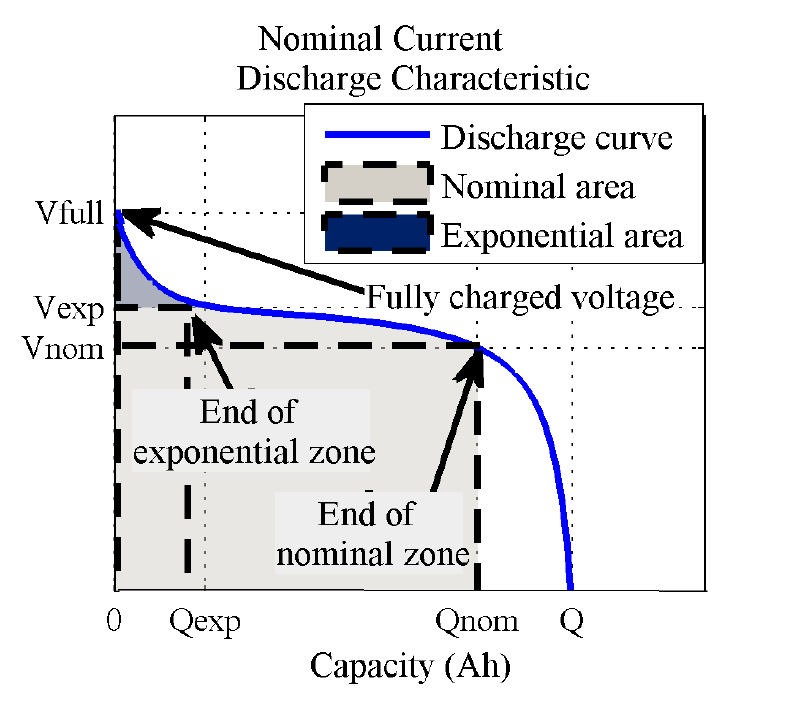
\includegraphics[scale=0.5]{images/Discharge.PNG}
	\label{abb:discharge_curve}
	\captionof{figure}{Typische Entladekurve für eine Batterie \cite{Tremblay.2009}}
\end{figure}
Für Li-Ion Batterien berechnet sich die Batteriespannung mit:
\begin{equation}
	V_{bat} = E_0-K\cdot\frac{Q}{Q-\int_{}^{} I_{bat} dt}\cdot\int_{}^{} I_{bat} dt - R\cdot I_{bat}+A\cdot e^{-3\cdot\int_{}^{} I_{bat} dt}-K\cdot\frac{Q}{Q-\int_{}^{} I_{bat} dt}\cdot i^* \label{eq:batteriespannung}
\end{equation}
mit 
\begin{description}
	\item \ensuremath{E_0} = konstante Batteriespannung
	\item \ensuremath{K} = Polarisationskonstante
	\item \ensuremath{Q} = Batteriekapazität
	\item \ensuremath{\int_{}^{} I_{bat} dt} = tatsächliche Batterieladung
	\item \ensuremath{A} = Amplitude der exponentiellen Zone
	\item \ensuremath{B} = inverse Zeitkonstante der exponentiellen Zone
	\item \ensuremath{R} = Innenwiderstand
	\item \ensuremath{i} = Batteriespannung
	\item \ensuremath{i^\star} = gefilterte Spannung (in diesem Fall \(= 0\))
\end{description}
Li-Po Batterien weisen ein der Li-Ion Batterie ähnliches Verhalten auf, weshalb beide nach \ref{eq:batteriespannung} berechnet werden können. Die unbekannten Batterieparameter können mit 3 diskreten Punkten für die Spannung pro Zelle \ensuremath{V_{full}}, \ensuremath{V_{exp}} und  \ensuremath{V_{nom}} und die Kapazität \ensuremath{Q}, \ensuremath{Q_{exp}} und \ensuremath{Q_{nom}} (vgl. Abb.\ref{abb:discharge_curve}) nach folgendem Schema
\begin{equation}
	\begin{pmatrix} E_0 \\ A \\ K \end{pmatrix} = A^{-1}\cdot \begin{pmatrix}
	V_{full}+R\cdot I_{bat} \\ V_{exp}+R\cdot I_{bat} \\ V_{nom}+R\cdot i \end{pmatrix}
\end{equation}
mit der Beziehung
\begin{equation}
	A = \begin{pmatrix}
	1 & 1 & 0 \\ 1 & e^{-3} & -\frac{Q\cdot (Q_{exp}+I_{bat})}{Q-Q_{exp}} \\ 1 & e^{-3\cdot\frac{Q_{nom}}{Q_{exp}}} & -\frac{Q\cdot (Q_{exp}+I_{bat})}{Q-Q_{exp}}
	\end{pmatrix}
\end{equation}
bestimmt werden.
Aus dieser Datenbank sind die oben genannten Punkte für die Spannung und Kapazität sowie die Innenwiderstände und Entladeströme angegeben. Die Punkte für die Spannung, $V_{full}, V_{exp} und V_{nom}$ entziehen sich einer Normierung, da sie bereits für nur eine Batteriezelle gelten. Die Punkte für die Kapazität und der Innenwiderstand beziehen sich allerdings auf die gesamte Batteriezelle. Daher ist eine Normierung auf eine Zelle notwendig, was mit dem arithmetischen Mittelwert geschieht. Dies ist jedoch für den Innenwiderstand zu ungenau, da er einen starken Einfluss auf die Genauigkeit des Modells hat und kleine Abweichungen zu eindeutigen Ungenauigkeiten führen. Für den Innenwiderstand kann ein Modell in Abhängigkeit der C-Rate und der Kapazität aufgestellt werden.  Die Abhängigkeit von beiden Faktoren zeigt ein hyperbolisches Verhalten auf was am besten durch einen Funktionstyp der Form 
\begin{equation}
	f(x,y) = \frac{k}{C_{Rate}\cdot(a\cdot C_{Rate}+b\cdot Q)^d}
\end{equation}
Beschrieben wird. Zur Steigerung der Genauigkeit, werden einige Batteriezellen aus der Berechnung der Erstellung dieses Modells herausgenommen, da diese erhebliche Abweichungen von der Standardabweichung aufzeigen. Hier sei angemerkt, dass sich dadurch die Genauigkeit vor allem  im Bereich kleiner C-Raten und Kapazitäten verringert.




%Interessant für die nachfolgende Untersuchungen ist eine Batteriezelle, die unabhängig vom Hersteller, der Kapazität, der Entladerate und anderen herstellerspezifischen Eigenheiten, verwendet werden kann.  Aus diesem Grund ist die Erstellung einer Normzelle von Interesse. Aus \textcolor{red}{Beyer2016a Blub} existiert bereits die Datenbank \texttt{Elektromodellflug} mit mehreren Batterien von unterschiedlichen Herstellern, in der alle benötigten Daten zur Erstellung dieser Zelle vorhanden sind. Ebenso existiert aus dieser Arbeit bereits eine Funktion zur Erstellung der in Abb.\ref{abb:discharge_curve} gezeigten Entladekurve. 
%Hierbei sind schon $V_{full}, V_{exp} und V_{nom}$ auf eine Zelle normiert, allerdings die anderen Parameter nicht. Folglich werden alle übrigen Parameter mit \SI{1}{Ah} normiert und der arithmetische Mittelwert über alle Batterien gebildet. Der Entladestrom entspricht dabei dem 1/100 der Batteriekapazität. 
%Erste Vergleich der normierten Zelle mit den ursprünglichen Batterien zeigten deutliche Unterschiede. Es wurde herausgefunden, dass der Innenwiderstand einen bedeutenden Einfluss auf die Abweichungen hat. Der arithmetische Mittelwert für den Widerstand ist an dieser zu Stelle zu ungenau. Dem Innenwiderstand in Abhängigkeit der Kapazität und der C-Rate kann einen hyperbolischen Verlauf in beide Richtungen zugrunde gelegt werden. Unter Vernachlässigung von Ausreißern können die Datenpunkte mit der Gleichung
%\begin{equation}
%	f(x,y) = \frac{k}{C_{Rate}\cdot(a\cdot x+b\cdot y)^d}
%\end{equation}
%angenähert werden. Hier sei angemerkt, dass durch das Entfernen von Batterien aus der Berechnung die Genauigkeit im Bereich kleiner C-Raten und Kapazitäten verringert. Nichtsdestotrotz ist damit die Genauigkeit in der Nähe der fixen Datenpunkte größer. Die Abweichungen der Batteriespannung des Modells von den realen Zellen sind in \textcolor{red}{Abb. Abweichungen} dargestellt. Dazu wurde jeweils die Fläche der Normzelle unter der Entladespannungskurve in Bezug zu der der tatsächlichen Batterie in Bezug gesetzt.

%Der Vergleich der berechneten Normzelle mit originalen Batterien teils starke Abweichungen von über \SI{100}{\%} von der ursprünglichen Batteriezelle. Zusätzlich wird der Einfluss der C-Rate auf diese Abweichungen mit berücksichtigt. Dabei kam heraus, dass gewisse Batterien signifikant von der angenäherten Zelle abweichen (z.B. Batterienummer 14,30,40 und 63). Diese wiesen deutliche Abweichungen von der mittleren Abweichung aller Zellen auf. Aus diesem Grund sind diese Batterien aus der Betrachtung entfernt und die Mittelwerte neu berechnet worden.


\subsection{Wirkungsgrad über das Gesamtsystem}
Zur Berechnung des Wirkungsgrads kann das Verhältnis der Leistung, die in Schub gewandelt wird zu der Leistung, die der Batterie entzogen wird, herangezogen werden
\begin{equation}
	\eta_{ges} = \frac{P_{Strahl}}{P_{Bat}}.
\end{equation}
Die Strahlleistung 
\begin{equation}
	P_{Strahl} = T\cdot (v_i + V_c)
\end{equation}
setzt sich aus dem Schub \ensuremath{T}, der induzierten Geschwindigkeit \ensuremath{v_i} und der Steiggeschwindigkeit \ensuremath{V_c} zusammen.
Zur Berechnung der induzierten Geschwindigkeit im Steigflug wird das Newton-Raphson-Verfahren herangezogen. Mit diesem lässt sich innerhalb weniger Iterationsschritte die induzierte Geschwindigkeit im Steigflug ermitteln \cite[S.153]{Wall.2015}:
\begin{equation}
	f(v) = v-\mu_z-\frac{{v_h}^2}{\sqrt{\mu^2+v^2}}
\end{equation}
\begin{equation}
	f'(v) = 1 + v\cdot\frac{{v_h}^2}{\sqrt{\mu^2+v^2}^3}
\end{equation}
\begin{equation}
	v_{n+1} = v_n - \frac{f(v_n)}{f'(v_n)}\qquad n = 0,1,2,\dots
\end{equation}
An dieser Stelle sei angemerkt, dass van der Wall mit dimensionslosen Durchflussgraden \ensuremath{\lambda} rechnet. In dieser Arbeit wird aber mit den dimensionsbehafteten Geschwindigkeiten gerechnet.
Der Startwert der Iteration ist die induzierte Geschwindigkeit im Schwebeflug
\begin{equation}
	v_h = \sqrt{\frac{m\cdot g}{2\cdot\rho\cdot A_{Rotor}\cdot n_{Prop}}}.
\end{equation}
Die der Batterie entzogenen Leistung
\begin{equation}
	P_{Bat} = U_{Bat}\cdot I_{Bat}
\end{equation}
ist das Produkt aus der Batteriespannung und -strom.


\subsection{Einhaltung leistungsbezogener Grenzen}
Für den Fall, dass technisch und aerodynamisch unmögliche Flugzustände erreicht werden, sind folgende technische und aerodynamische Grenzen festgelegt:
\begin{itemize}
	\item Die Restladung im Steigflug ist kleiner als  Null oder kleiner als eine vorher festgelegte, minimale Restkapazität (Kapazität der Batterie reicht nicht aus oder zu hohe Flugzeit)
	\item Die Motorspannung ist größer als die nominelle Spannung der Batterie bzw. die PWM ist größer als \SI{100}{\%} (zu hohe Winkelgeschwindigkeit im Steigflug erforderlich)
	\item Die Motorspannung oder der Motorstrom ist kleiner/gleich Null (physikalisch unmöglicher Steigflug oder zu schneller Sinkflug)
	\item Die C-Rate ist größer als die maximal zulässige C-Rate der Batterie (Batterieentladestrom ist höher als zulässig)
	\item Der Motorstrom ist höher als der maximal zulässige Dauerstrom des Motors unter Last (zu hohes Drehmoment gefordert)
	\item Der lokale Anstellwinkel überschreitet den festgelegten Grenzwert von \ensuremath{\alpha_{max}}(Strömungsabriss)
	\item Die Blattspitzengeschwindigkeit überschreitet \ensuremath{M_{tip}=1}(transsonische Strömung)
	\item Der Gesamtwirkungsgrad ist größer als \SI{100}{\%} (ein physikalisch unmöglicher Zustand)
	\item Die Restladung nimmt zu \ensuremath{Restladung_{i+1} > Restladung_{i}} (ein physikalisch nicht erreichbarer Zustand für diese Bestrachtung)
\end{itemize}

\section{Vernachlässigungen und Vereinfachungen}
\label{sec:vernachlaessigungen_vereinfachungen}

\subsection{Einschränkungen}
Für die Leistungsberechnung sind mehrere Vernachlässigungen vorzunehmen. Zuerst wurden keinerlei dynamische Effekte und Verhalten berücksichtigt. Dies beinhaltet translatorische Beschleunigungen des Multicopters, rotatorische Beschleunigungen der Rotoren zum Störausgleich sowie und rotatorische Beschleunigungen des Multicopters durch Ungenauigkeiten des Lagereglers. Das gleiche gilt für das Flächenflugzeug. 
Die Störgrößen, in diesem Fall vor allem der laterale Seitenwind, werden als statisch und konstant vorausgesetzt. Hierbei werden jegliche Veränderungen des Windes und Böen mit der Höhe vernachlässigt. Auf- und Abwinde entziehen sich auch der Betrachtung. Hinzu kommt die Vernachlässigung der Totzeit des Reglers. 
Weiterhin nicht berücksichtigt bleiben Reynoldszahl- und Machzahleffekte. Transonische Strömung unterhalb einer Blattspitzengeschwindigkeit von \ensuremath{M_{tip}=1} kann aus diesem Grund nicht ausgeschlossen werden.
Die ganze Leistung der Batterie geht in diesem Modell ausschließlich in die Schuberzeugung. Das heißt, dass die Regler und sonstige elektrische Komponenten keinen zusätzlichen Strom verbrauchen.
Das Flächenflugzeug wird in dem Programm als eine Punktmasse ohne Abmaße betrachtet. Um eine möglichst allgemeine Dimensionierung eines Flugsystems mit fixed wings zu ermöglichen wird sich hier jeglicher genauerer Beschreibungen des Systems verwehrt. So wird auf Kennzahlen wie die Streckung, die Flügelfläche oder z.B. Auftriebs- und Widerstandsbeiwerten verzichtet. Dies zieht eine derartige Betrachtung des Systems mit sich, dass nur der Einfluss von Gleitzahl, Motorisierung und anderen Einflussfaktoren betrachtet werden. Eine exakte Auslegung kann deshalb nur im Anschluss vorgenommen werden. Diese Vereinfachungen müssen in der Auswertung berücksichtigt werden.

\subsection{Vereinfachungen}
\subsubsection{Schub}
Der Schub wird innerhalb eines sehr einfachen Modells berechnet. Das gilt sowohl für den Multicopter als auch für das Flächenflugzeug. Der Multicopter ist als eine Art Rotationsellipsoid und das Flächenflugzeug als Punktmasse vereinfacht

\subsubsection{Propeller und Kennfeld}
Bei der Transformation der Propellerkennfelder auf äquidistante Geschwindigkeitsabstände ist der Bereich von \SI{-10}{m/s} bis \SI{0}{m/s} extrapoliert. Ein analoges Vorgehen wird zur Erweiterung des ursprünglichen Kennfeldes in den Bereich noch größerer Anströmgeschwindigkeiten angewandt. Das reale Verhalten der Propeller kann folglich von dem errechneten abweichen. Weiterhin beziehen sich alle Auslegungen auf die Datenbank von APC. 
Die Modellierung eines Propellers mit gleichem Durchmesser und gleicher Steigung eines anderen Herstellers kann aus diesem Grund abweichen. Gründe dafür können eine unterschiedliche Profilierung, Verwindung oder Profiltiefenverteilung sein. 

\subsubsection{Motor}
Jeglicher Einfluss der Temperatur auf die Leistung des Motors bleibt in dem einfachen Motormodell unberücksichtigt. Außerdem werden der Motorstrom und der der Innenwiderstand als konstant angenommen.

\subsubsection{Motorregler}
Für den Motorregler wurde ein sehr einfaches Modell verwendet, in dem der Wirkungsgrad ausschließlich eine Funktion der PWM ist.

\subsubsection{Batterie}
Die Berechnung der Batterie vernachlässigt zwei wichtige Einflussfaktoren. Das ist der Temperatureinfluss und der Einfluss der Alterung auf die Kapazität. Dies kann jedoch durch eine Anpassung der Peukert-Konstante kompensiert werden.\\
Zusätzlich unterliegt die Batteriespannung im Rahmen des Modells Abweichungen. Diese nehmen für zunehmende C-Raten ebenfalls zu (Vgl. Abb. \ref{abb:abweichungen}). In diesem ist das Verhältnis der Flächen unterhalb der Spannungskurve von der normierten Batteriezelle zur Originalzelle aufgetragen (\ensuremath{V_{Bat,normiert}/V_{Bat,original}}. Für die Berechnung der Abweichungen werden Batterien, deren maximale C-Rate bereits überschritten ist, herausgenommen. Außerdem werden Batterien in der Berechnung nicht berücksichtigt, deren individuelle Abweichung eine große Diskrepanz zur Standardabweichung aufweist. Die Genauigkeit des Modells steigt somit. Im unteren Diagramm von Abb. \ref{abb:abweichungen} ist beispielhaft die Spannungsabweichung jeder normierten Zelle von der Originalzelle sowie die Standardabweichung dargestellt.
\begin{figure}[H]
\centering
	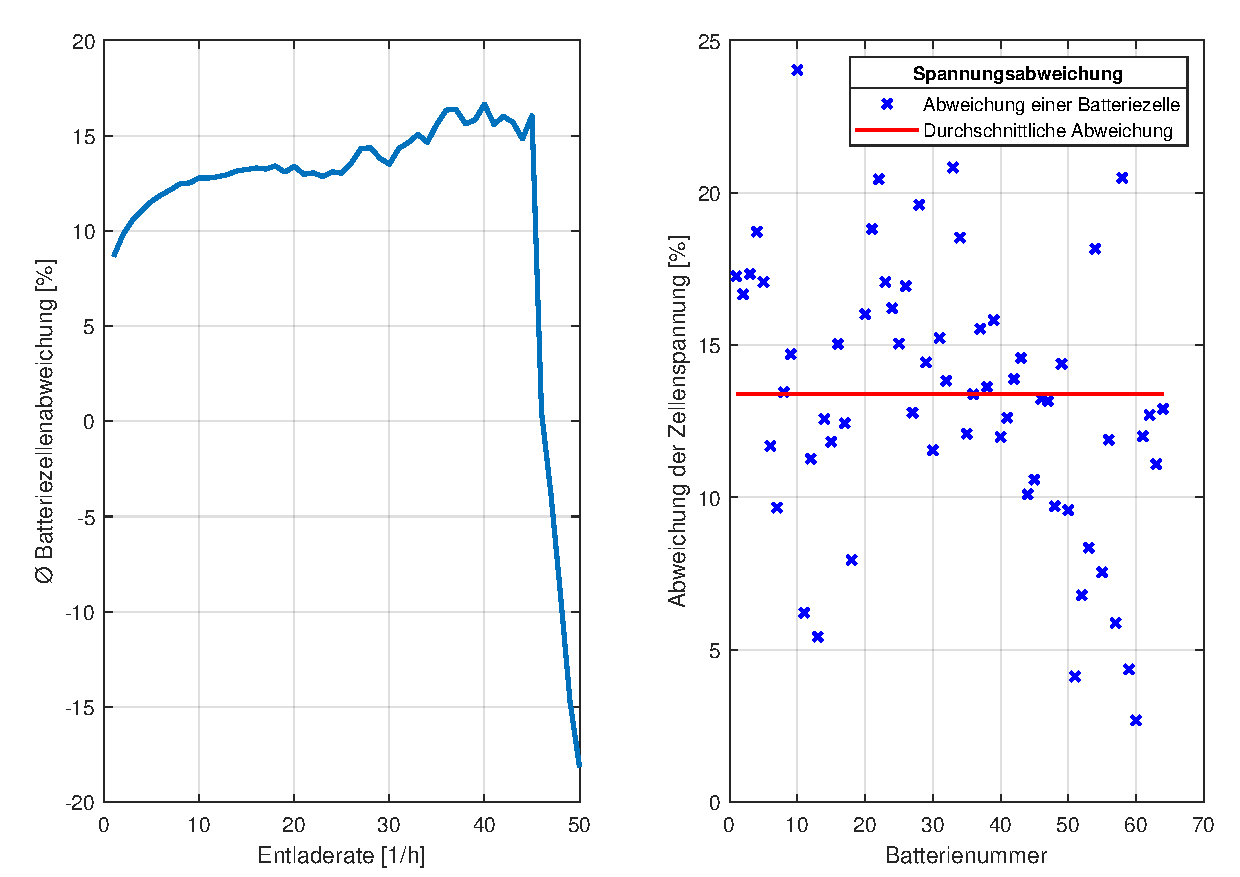
\includegraphics{Diagramme/Abweichungen.pdf}
	\caption{oben: Durschnittliche Spannungsabweichungen der Normzelle von den Zellen aus der Batteriedatenbank in Abhängigkeit von der C-Rate, \\
	unten: Beispiel für die Spannungsabweichungen jeder Normzelle im Vergleich zur Originalzelle für eine C-Rate von 20 (\texttt{PWM}=0.8, \texttt{eta\_PWM}=0.7, \texttt{I\_mot}=8, \texttt{n\_Prop}=4)}
	\label{abb:abweichungen}
\end{figure}
Die Zuverlässigkeit des Batteriemodells nimmt daher mit hohen C-Raten ab. Außerdem ist zu berücksichtigen, dass im Durchschnitt der Spannungsverlauf der normierten Zelle unterhalb der Normalzelle liegt. Dies bedeutet, dass die Spannung der Originalzelle unter Last geringer einbricht, als die der normierten Zelle.  

\subsubsection{Wirkungsgrad}
Die Berechnung der Strahlleistung beruht auf der Berechnung der induzierten Geschwindigkeit innerhalb der Strahltheorie. Hier wird ein idealer Rotor zugrunde gelegt.
Beruhend auf dieser Annahme bleiben viele Effekte wie Blattspitzeffekte an der Rotorblattspitze und im Bereich der Rotorblattaufhängung, Strömungsablösungen, Blattwirbelinteraktionen usw. unberücksichtigt.  Zudem wird eine über den Radius konstante induzierte Geschwindigkeit in der Rotorebene angenommen. Dies ist im Vorwärtsflug und bei Schräganströmung zu relativieren \cite[S.226]{Wall.2015}.
